%%% The main file. It contains definitions of basic parameters and includes all other parts.

%% Settings for single-side (simplex) printing
% Margins: left 40mm, right 25mm, top and bottom 25mm
% (but beware, LaTeX adds 1in implicitly)
\documentclass[12pt,a4paper]{report}
\setlength\textwidth{145mm}
\setlength\textheight{247mm}
\setlength\oddsidemargin{15mm}
\setlength\evensidemargin{15mm}
\setlength\topmargin{0mm}
\setlength\headsep{0mm}
\setlength\headheight{0mm}
% \openright makes the following text appear on a right-hand page
\let\openright=\clearpage

%% Settings for two-sided (duplex) printing
% \documentclass[12pt,a4paper,twoside,openright]{report}
% \setlength\textwidth{145mm}
% \setlength\textheight{247mm}
% \setlength\oddsidemargin{14.2mm}
% \setlength\evensidemargin{0mm}
% \setlength\topmargin{0mm}
% \setlength\headsep{0mm}
% \setlength\headheight{0mm}
% \let\openright=\cleardoublepage

%% Generate PDF/A-2u
\usepackage[a-2u]{pdfx}

%% Character encoding: usually latin2, cp1250 or utf8:
\usepackage[utf8]{inputenc}

%% Prefer Latin Modern fonts
\usepackage{lmodern}

%% Further useful packages (included in most LaTeX distributions)
\usepackage{amsmath}        % extensions for typesetting of math
\usepackage{amsfonts}       % math fonts
\usepackage{amsthm}         % theorems, definitions, etc.
\usepackage{bbding}         % various symbols (squares, asterisks, scissors, ...)
\usepackage{bm}             % boldface symbols (\bm)
\usepackage{graphicx}       % embedding of pictures
\usepackage{fancyvrb}       % improved verbatim environment
\usepackage{natbib}         % citation style AUTHOR (YEAR), or AUTHOR [NUMBER]
\usepackage[nottoc]{tocbibind} % makes sure that bibliography and the lists
			    % of figures/tables are included in the table
			    % of contents
\usepackage{dcolumn}        % improved alignment of table columns
\usepackage{booktabs}       % improved horizontal lines in tables
\usepackage{paralist}       % improved enumerate and itemize
\usepackage{xcolor}         % typesetting in color

%% SPECIMEN
% Parts marked as SPECIMEN are used for building the example PDF.
% When the official template is generated by ./mkdist, all such parts
% are deleted, as well as all calls of \X and \XXX macros.
\def\X#1{\textcolor{red}{[#1]}}
\def\XXX#1{\par\smallskip\noindent \textcolor{red}{[#1]}}
%% NEMICEPS

%%% Basic information on the thesis

% Thesis title in English (exactly as in the formal assignment)
\def\ThesisTitle{Thesis title \X{as in the formal assignment}}

% Author of the thesis
\def\ThesisAuthor{Jana Bátoryová}

% Year when the thesis is submitted
\def\YearSubmitted{2020}

% Name of the department or institute, where the work was officially assigned
% (according to the Organizational Structure of MFF UK in English,
% or a full name of a department outside MFF)
\def\Department{Name of the department \X{as per Organizational Structure of MFF UK in English}}

% Is it a department (katedra), or an institute (ústav)?
\def\DeptType{Department}

% Thesis supervisor: name, surname and titles
\def\Supervisor{Supervisor's Name \X{+titles}}

% Supervisor's department (again according to Organizational structure of MFF)
\def\SupervisorsDepartment{department}

% Study programme and specialization
\def\StudyProgramme{study programme}
\def\StudyBranch{study branch}

% An optional dedication: you can thank whomever you wish (your supervisor,
% consultant, a person who lent the software, etc.)
\def\Dedication{%
Dedication.
}

% Abstract (recommended length around 80-200 words; this is not a copy of your thesis assignment!)
\def\Abstract{%
Abstract. \X{Recommended length around 80--200 words. This is not a~copy of your thesis assignment!}
}

% 3 to 5 keywords (recommended), each enclosed in curly braces
\def\Keywords{%
{key} {words} \X{usually 3 to~5 key words or phrases}
}

%% The hyperref package for clickable links in PDF and also for storing
%% metadata to PDF (including the table of contents).
%% Most settings are pre-set by the pdfx package.
\hypersetup{unicode}
\hypersetup{breaklinks=true}

% Definitions of macros (see description inside)
%%% This file contains definitions of various useful macros and environments %%%
%%% Please add more macros here instead of cluttering other files with them. %%%

%%% Minor tweaks of style

% These macros employ a little dirty trick to convince LaTeX to typeset
% chapter headings sanely, without lots of empty space above them.
% Feel free to ignore.
\makeatletter
\def\@makechapterhead#1{
  {\parindent \z@ \raggedright \normalfont
   \Huge\bfseries \thechapter. #1
   \par\nobreak
   \vskip 20\p@
}}
\def\@makeschapterhead#1{
  {\parindent \z@ \raggedright \normalfont
   \Huge\bfseries #1
   \par\nobreak
   \vskip 20\p@
}}
\makeatother

% This macro defines a chapter, which is not numbered, but is included
% in the table of contents.
\def\chapwithtoc#1{
\chapter*{#1}
\addcontentsline{toc}{chapter}{#1}
}

% Draw black "slugs" whenever a line overflows, so that we can spot it easily.
\overfullrule=1mm

%%% Macros for definitions, theorems, claims, examples, ... (requires amsthm package)

\theoremstyle{plain}
\newtheorem{thm}{Theorem}
\newtheorem{lemma}[thm]{Lemma}
\newtheorem{claim}[thm]{Claim}

\theoremstyle{plain}
\newtheorem{defn}{Definition}

\theoremstyle{remark}
\newtheorem*{cor}{Corollary}
\newtheorem*{rem}{Remark}
\newtheorem*{example}{Example}

%%% An environment for proofs

\newenvironment{myproof}{
  \par\medskip\noindent
  \textit{Proof}.
}{
\newline
\rightline{$\qedsymbol$}
}

%%% An environment for typesetting of program code and input/output
%%% of programs. (Requires the fancyvrb package -- fancy verbatim.)

\DefineVerbatimEnvironment{code}{Verbatim}{fontsize=\small, frame=single}

%%% The field of all real and natural numbers
\newcommand{\R}{\mathbb{R}}
\newcommand{\N}{\mathbb{N}}

%%% Useful operators for statistics and probability
\DeclareMathOperator{\pr}{\textsf{P}}
\DeclareMathOperator{\E}{\textsf{E}\,}
\DeclareMathOperator{\var}{\textrm{var}}
\DeclareMathOperator{\sd}{\textrm{sd}}

%%% Transposition of a vector/matrix
\newcommand{\T}[1]{#1^\top}

%%% Various math goodies
\newcommand{\goto}{\rightarrow}
\newcommand{\gotop}{\stackrel{P}{\longrightarrow}}
\newcommand{\maon}[1]{o(n^{#1})}
% \newcommand{\abs}[1]{\left|{#1}\right|}
\newcommand{\dint}{\int_0^\tau\!\!\int_0^\tau}
\newcommand{\isqr}[1]{\frac{1}{\sqrt{#1}}}

%%% Various table goodies
\newcommand{\pulrad}[1]{\raisebox{1.5ex}[0pt]{#1}}
\newcommand{\mc}[1]{\multicolumn{1}{c}{#1}}


% Title page and various mandatory informational pages
\begin{document}
%%% Title page of the thesis and other mandatory pages

%%% SPECIMEN
%%% Inscriptions at the opening page of the hard cover

\pagestyle{empty}
\hypersetup{pageanchor=false}
\XXX{Opening page of the hard cover. Not a part of the electronic version.}
\begin{center}

\large
Charles University

\medskip

Faculty of Mathematics and Physics

\vfill

{\huge\bf BACHELOR THESIS}

\vfill

\hbox to \hsize{\YearSubmitted\hfil \ThesisAuthor}

\end{center}

\newpage\openright

%%% NEMICEPS

%%% Title page of the thesis

\pagestyle{empty}
\hypersetup{pageanchor=false}
\begin{center}

\centerline{\mbox{
\includegraphics[width=166mm]{img/logo-en.pdf}}}

\vspace{-8mm}
\vfill

{\bf\Large BACHELOR THESIS}

\vfill

{\LARGE\ThesisAuthor}

\vspace{15mm}

{\LARGE\bfseries\ThesisTitle}

\vfill

\Department

\vfill

{
\centerline{\vbox{\halign{\hbox to 0.45\hsize{\hfil #}&\hskip 0.5em\parbox[t]{0.45\hsize}{\raggedright #}\cr
Supervisor of the bachelor thesis:&\Supervisor \cr
\noalign{\vspace{2mm}}
Study programme:&\StudyProgramme \cr
\noalign{\vspace{2mm}}
Study branch:&\StudyBranch \cr
}}}}

\vfill

% Zde doplňte rok
Prague \YearSubmitted

\end{center}

\newpage

%%% NOPHD
%%% Here should be a bound sheet included -- a signed copy of the "bachelor
%%% thesis assignment". This assignment is NOT a part of the electronic
%%% version of the thesis. DO NOT SCAN.
\XXX{Bound into the introductory part must be the form with signed approval of the thesis topic (a photocopy suffices).
This is not a~part of the electronic version of the thesis, do not scan!}
%%% PHDNO

%%% A page with a solemn declaration to the bachelor thesis

\openright
\hypersetup{pageanchor=true}
\pagestyle{plain}
\pagenumbering{roman}
\vglue 0pt plus 1fill

\noindent
I declare that I carried out this bachelor thesis independently, and only with the cited
sources, literature and other professional sources. It has not been used to obtain another
or the same degree.

\medskip\noindent
I understand that my work relates to the rights and obligations under the Act No.~121/2000 Sb.,
the Copyright Act, as amended, in particular the fact that the Charles
University has the right to conclude a license agreement on the use of this
work as a school work pursuant to Section 60 subsection 1 of the Copyright~Act.

\vspace{10mm}

\hbox{\hbox to 0.5\hsize{%
In \hbox to 6em{\dotfill} date \hbox to 6em{\dotfill}
\hss}\hbox to 0.5\hsize{\dotfill\quad}}
\smallskip
\hbox{\hbox to 0.5\hsize{}\hbox to 0.5\hsize{\hfil Author's signature\hfil}}

\vspace{20mm}
\newpage

%%% Dedication

\openright

\noindent
\Dedication

\newpage

%%% Mandatory information page of the thesis

\openright

\vbox to 0.5\vsize{
\setlength\parindent{0mm}
\setlength\parskip{5mm}

Title:
\ThesisTitle

Author:
\ThesisAuthor

\DeptType:
\Department

Supervisor:
\Supervisor, \SupervisorsDepartment

Abstract:
\Abstract

Keywords:
\Keywords

\XXX{This information must be stored as PDF meta-data, too. Please refer to the {\tt README} file.}
\vss}

\newpage

\openright
\pagestyle{plain}
\pagenumbering{arabic}
\setcounter{page}{1}


%%% A page with automatically generated table of contents of the bachelor thesis

\tableofcontents

%%% Each chapter is kept in a separate file
\chapter*{Introduction}
\addcontentsline{toc}{chapter}{Introduction}




\chapter{Preliminaries}

\section{Deep Learning}

\subsection{Deep Neural Network Features}

Deep Neural Networks are composed of layers. These stacked layers on top of each other transfer sequentially information from the beginnning until the end. Several researches showed the ability of different layers percieving different type of information. The high level features are build on top of low level features, detected in the early layers. Therefore, the layers have descriptive power. Later in this thesis, we use the features from penultimate and antepenultimate layers of common image recognition Depp Neural Networks.

\begin{figure}
	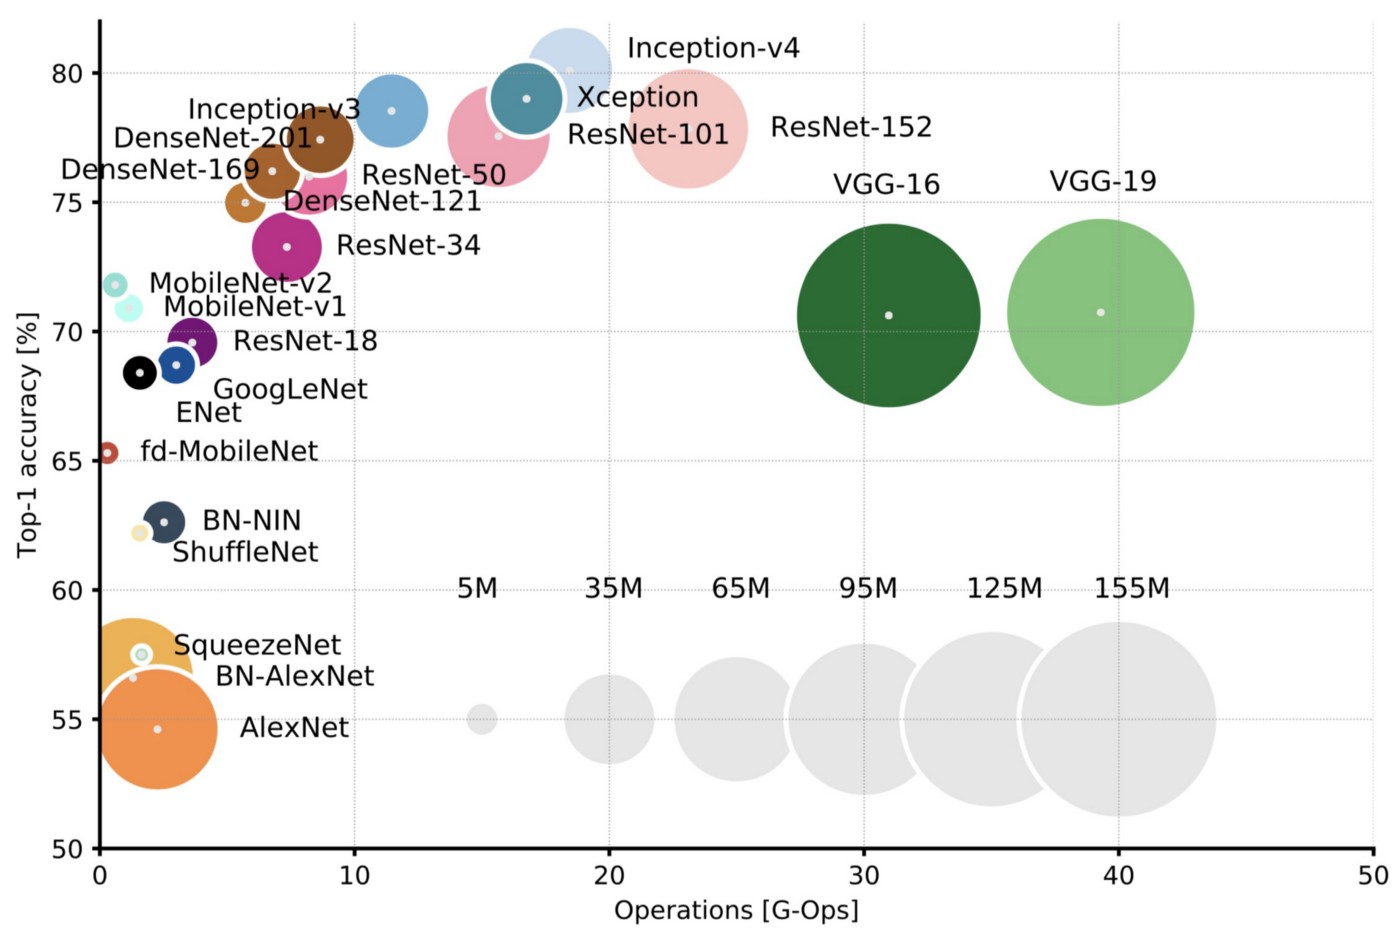
\includegraphics[width=0.8\linewidth]{img/network-comparison.jpeg}
	\caption{Comparison of widely used Image Recognition networks and their performance. Src:TODO: https://arxiv.org/abs/1605.07678}
	\label{fig:camera-setup}
\end{figure}


\section{Distance Measures}

\subsection{Cosine Distance}
\begin{equation}
similarity = \cos ({\bf t},{\bf e})= {{\bf t} {\bf e} \over \|{\bf t}\| \|{\bf e}\|} = \frac{ \sum_{i=1}^{n}{{\bf t}_i{\bf e}_i} }{ \sqrt{\sum_{i=1}^{n}{{\bf t}_i^2}} \sqrt{\sum_{i=1}^{n}{{\bf e}_i^2}} }
\end{equation}
\begin{equation}
    distance = 1 - similarity
\end{equation}

\subsection{Euclidean Distance}
\begin{equation}
d(p, q) = \sqrt{\sum_{i=1}^n (p_i - q_i)^2}    
\end{equation}

\section{Self organizing maps}

\section{?Clustering}

\section{Dataset}

\chapter{Search by Object Location}

First approach we explore is based on knowing the position of the objects in the image. This corresponds to a visual memory. People with a good visual memory are usually able to describe the position of the objects regarding to each other or in absolute way in the whole image. An example to this shows the image \todo[]{}.

We aim to overcome a limitation on vocabulary size for common approach by description of words. We implement search only on visual requests, which, if takes rich enoucgh descriptors has significantly higher capability.

\todo[inline]{Obrazok s hladanou scenou dvoch ludi a k tomu vsetkymi obrazkami kde su dvaja ludia}
\todo[inline]{Obrazok s hladanou scenou dvoch ludi a k tomu kolaz ktora zobrazuje ewquest}

\todo[inline]{Motivation --  spomienka toho, ako vyzerala scena}
\todo[inline]{Now we present following two approaches...}
In the TrackVid competition, many presented solutions are limited and do not scale well. For example is keyword search, which is limited to the size of the vocabulary. In this chapter we overcome this limitation. We develop search based on images instead of words to avoid the vocabulary limit. We use state-of-art knowledge to acquire deep representation of the objects.

The second limitation we tackle is multi-query. It is difficult to find a source video if many scenes with the same type of the objects occur in the dataset (see Image ....). We solve this problem by placing multiple single queries and then using fusion to merge rankings from each query (more in ...).


The research in the recent years showed, that neural networks purposfully trained for a set of objects can gain an ability to create a good representation also for unseen objects \todo[]{source}. In this thesis we work with this presumption and we work with these representations.

\section{Visual Descriptor}
\section{Deep Visual Representations}
--- obfuskavanie sieti

\section{Query}

The query is a collage of one or multiple images. Each image also includes its relative position in the canvas.

The user interacts with the environemnt by adding, scaling and moving images. Interactively, closest representatives found in the dataset are returned. The user can submit if he successfully found the searched scene. The number of hints are taken into account.

The image \todo[]{query image} shows an example of our query. The goal is to be able to use any of currently available image search engines to create a collage. The user places multiple images on the canvas. Their position on the canvas is recorded and later used to target the database in regard to their position. 


\section{Splitting an Image into Regions}



In our first approach we cut the image into fixed regions. We aim to capture the 
representation of each of these regions. This offers us an information specific for each region.

With the query we can compare the features representation of the query and of the particular regions we are interested in.

Image
- Split to nxm regions
- Compute deep representation for each of the regions

Query
compute deep representation for the image in the query
for each image in the database, compare this representation to the representation of the region with highest IoU


In our first approach we split the image to a regions. We compute a deep representation using neural network for each region and the whole image. 
\section{ Using Deep Representation}
   - Using Deep Representation
      = Using antepenultimate layer of classification networks

\section{Multi-query search}
- Multi query search
  - Fusion methods
  - Comparison of both approaches with multimodal performance over different fusion techniques

Our work focuses on difficult to describe scenes with multiple easy to recognize objects. In this questions a natural question of how to rank the results based on multi query.

In this section we go through several approaches we tested. We base our 

\subsection{Fusion Methods}

\section{Evaluation}
In this chapter we evaluate all previously mentioned approached. Firstly, we describe our methodology behind the experiments and then we proceed through all approaches. 

\chapter{Search by Face Similarity}

Research in past several decades proved that human have extreme capability of recognizing the faces. Faces are so special to us as a species, that we are able to ..... We are able to recall that we met specific person dating the meeting years back. Therefore we state a question, if the search based only on faces can be done.

This approach organizes the space of seen faces to help the user to orientate and find the search face. Though, in order to describe the face space we use deep encodings trained by a network used for face recognition.

In the previous chapter we elaborated an approach to search in dataset using objects and their spatial information. In this chapter we investigate a different option -- traversion using faces. The question we ask is if it is possible to find a specific scene by showing user faces. Since there is a limitation of how many faces we can display at once to the user, we will investigate if we can lead user to the specific scene with specific face via traversion through multiple similar faces.

Since the similarity of faces is a strongly abstract perception we rely on feature representation of the faces. This helps us to create an interactive environment to traverse via huge aount of faces and test our hypothesis, if this approach can be used for scene searching. 

This chapter firstly introduces different approaches to obtaining face representations. Then we proceed by presenting different approaches for traversion over dataset of faces. At the end of the chapter we present the results in our specific task -- scene search .

\todo[inline]{ motivation - otestovat hypotezu ci je to mozne a nejaky nahlad ako ot moze vyzerat}
\section{Preliminaries}
\todo[inline]{face features - popisat zdroj siete}
\section{Creating SOM Representation of the face space}
\section{Evaluation}

Appendix
\chapter{User Guide (how to use the app to search)}
\chapter{ Running the app on the new set of images}
\todo[inline]{kde zmenit data a co znova natrenovat}
\chapter{Experiments evaluation (ako ziskat vysledky znova)}
\chapter{Code Structure (programmer's guide)}


% Searching Image Collections Using Deep Representations of Local Regions

% The thesis will investigate two particular approaches for searching large video datasets. The first approach will try to retrieve a searched scene based on a query collage consisting of example images organized on a canvas. The author will investigate various fusion methods, taking into account also the canvas positioning of the query images.  The second approach will be designed to search for a scene based on faces available in the dataset. The method will be based on visual exploration of the faces based on their similarities. In exploration approaches, the user can choose a similar face to the searched one, and continuously browse towards the searched face. The author will provide an interactive search environment for querying as a part of the solution and evaluate the recall on sets of experiments to estimate, how successfully users can retrieve particular scenes.


% \chapter{Title of the second chapter}

\section{Title of the first subchapter of the second chapter}

\section{Title of the second subchapter of the second chapter}


\chapter*{Conclusion}
\addcontentsline{toc}{chapter}{Conclusion}


%%% Bibliography
%%% Bibliography (literature used as a source)
%%%
%%% We employ bibTeX to construct the bibliography. It processes
%%% citations in the text (e.g., the \cite{...} macro) and looks up
%%% relevant entries in the bibliography.bib file.
%%%
%%% The \bibliographystyle command selects, which style will be used
%%% for references from the text. The argument in curly brackets is
%%% the name of the corresponding style file (*.bst). Both styles
%%% mentioned in this template are included in LaTeX distributions.

\bibliographystyle{plainnat}    %% Author (year)
% \bibliographystyle{unsrt}     %% [number]

\renewcommand{\bibname}{Bibliography}

%%% Generate the bibliography. Beware that if you cited no works,
%%% the empty list will be omitted completely.

\bibliography{bibliography}

%%% If case you prefer to write the bibliography manually (without bibTeX),
%%% you can use the following. Please follow the ISO 690 standard and
%%% citation conventions of your field of research.

% \begin{thebibliography}{99}
%
% \bibitem{lamport94}
%   {\sc Lamport,} Leslie.
%   \emph{\LaTeX: A Document Preparation System}.
%   2nd edition.
%   Massachusetts: Addison Wesley, 1994.
%   ISBN 0-201-52983-1.
%
% \end{thebibliography}


%%% Figures used in the thesis (consider if this is needed)
\listoffigures

%%% Tables used in the thesis (consider if this is needed)
%%% In mathematical theses, it could be better to move the list of tables to the beginning of the thesis.
\listoftables
\XXX{In mathematical theses, it could be better to move the list of tables to the beginning of the thesis.}

%%% Abbreviations used in the thesis, if any, including their explanation
%%% In mathematical theses, it could be better to move the list of abbreviations to the beginning of the thesis.
\chapwithtoc{List of Abbreviations}
\XXX{In mathematical theses, it could be better to move the list of abbreviations to the beginning of the thesis.}

%% PHDONLY
%%% Doctoral theses must contain a list of author's publications
\chapwithtoc{List of publications}
\XXX{Doctoral theses must contain a list of author's publications.}
%% ONLYPHD

%%% Attachments to the bachelor thesis, if any. Each attachment must be
%%% referred to at least once from the text of the thesis. Attachments
%%% are numbered.
%%%
%%% The printed version should preferably contain attachments, which can be
%%% read (additional tables and charts, supplementary text, examples of
%%% program output, etc.). The electronic version is more suited for attachments
%%% which will likely be used in an electronic form rather than read (program
%%% source code, data files, interactive charts, etc.). Electronic attachments
%%% should be uploaded to SIS and optionally also included in the thesis on a~CD/DVD.
%%% Allowed file formats are specified in provision of the rector no. 72/2017.
\appendix
\chapter{Attachments}
\XXX{Attachments to the bachelor thesis, if any. Each attachment must be referred to at least once from the text of the thesis. Attachments are numbered.}
\XXX{The printed version should preferably contain attachments, which can be read (additional tables and charts, supplementary text, examples of program output, etc.). The electronic version is more suited for attachments which will likely be used in an electronic form rather than read (program source code, data files, interactive charts, etc.). Electronic attachments should be uploaded to SIS and optionally also included in the thesis on a~CD/DVD. Allowed file formats are specified in provision of the rector no. 72/2017.}

\section{First Attachment}

\openright
\end{document}
